\documentclass[main.tex]{subfiles}
\begin{document}

\href{https://www2.seas.gwu.edu/~simhaweb/quantum/modules/module6/module6.html}{Module 6: Quantum Circuits - Gates}\\
\href{https://www2.seas.gwu.edu/~simhaweb/quantum/modules/module6/problems6.html}{Module-6 Solved Problems}

\begin{enumerate}

\item[] \textbf{In-Class Exercise 1:} Use the Dirac form and
\begin{enumerate}
    \item [1.] \textbf{Q.} Show that $Y(\alpha|0\rangle+\beta|1\rangle)=i(\alpha|1\rangle-\beta|0\rangle)$ \textbf{A.}
    \begin{align*}
        Y(\alpha|0\rangle + \beta |1\rangle)    & = (-i|0\rangle\langle1| + i|1\rangle\langle0|)
                                                (\alpha|0\rangle + \beta |1\rangle)\\
                                                & = -i\beta|0\rangle + i\alpha|1\rangle\\
                                                & = i(\alpha|1\rangle-\beta|0\rangle)
    \end{align*}        
    \item [2.] \textbf{Q.} Show that $Y$ switches the Hadamard basis vectors. (Remember global phase.) \textbf{A.}
    \begin{align*}
        Y|+\rangle  & = (-i|0\rangle\langle 1|+i| 1\rangle\langle 0|)\frac{1}{\sqrt{2}}(|0\rangle + |1\rangle)\\
                    & = \frac{i}{\sqrt{2}}(|0\rangle - |1\rangle)\\
                    & = i|-\rangle\\
        Y|-\rangle  & = (-i|0\rangle\langle 1|+i| 1\rangle\langle 0|)\frac{1}{\sqrt{2}}(|0\rangle - |1\rangle)\\
                    & = \frac{i}{\sqrt{2}}(|0\rangle + |1\rangle)\\
                    & = i|+\rangle\\
    \end{align*}
\end{enumerate}

\item[] \textbf{In-Class Exercise 2:} \textbf{Q.} Prove the identity $YZ=-ZY=iX$ \textbf{A.}
    \begin{align*}
        YZ  & = (-i|0\rangle\langle1| + i|1\rangle\langle0|)(|0\rangle\langle0| - |1\rangle\langle1|)\\
            & = i|0\rangle\langle1| + i|1\rangle\langle 0|\\
            & = -(|0\rangle\langle0| - |1\rangle\langle1|)(-i|0\rangle\langle1| + i|1\rangle\langle0|)\\
            & = -ZY\\
            & = i|0\rangle\langle1| + i|1\rangle\langle 0|\\
            & = iX
    \end{align*}

\item[] \textbf{In-Class Exercise 3:} \textbf{Q.} Derive the matrix for $R_{Z}(\theta)$ and show that it is unitary. Is it Hermitian? \textbf{A.}
    \begin{align*}
        R_{Z}(\theta)               & = e^{\frac{-i \theta}{2} Z}\\
                                    & = I\cos \frac{\theta}{2} - i Z\sin\frac{\theta}{2}\\
                                    & = \cos\frac{\theta}{2}\left[\begin{array}{ll}1&0\\0&1\end{array}\right]
                                    -\sin\frac{\theta}{2}\left[\begin{array}{ll}i&0\\0&-i\end{array}\right]\\
                                    & = \left[\begin{array}{cc}e^{\frac{-i \theta}{2}} & 0 \\ 
                                    0 & e^{\frac{i \theta}{2}}\end{array}\right]\\
        \left[\begin{array}{ll}
        e^{\frac{-i \theta}{2}}&0\\ 
        0 & e^{\frac{i \theta}{2}}
        \end{array}\right]
        \left[\begin{array}{ll}
        e^{\frac{-i \theta}{2}}&0\\ 
        0 & e^{\frac{i \theta}{2}}
        \end{array}\right]^*        & = \left[\begin{array}{ll}e^0&0\\0&e^0\end{array}\right]\\
                                    & = I\\
        R_{Z}(\theta)^{\dagger}     & = \left[\begin{array}{ll}e^{\frac{i \theta}{2}}&0\\
                                    0 & e^{\frac{-i \theta}{2}}\end{array}\right]\\
                                    & \neq R_{Z}(\theta)
    \end{align*}
    $R_{Z}(\theta)$ is not Hermitian.
    
\item[] \textbf{In-Class Exercise 4:} \textbf{Q.} Show that the three operators $T, R, K$ commute with different parameters: \textbf{A.}
\begin{enumerate}
    \item [1.] $T\left(\alpha_{1}\right) T\left(\alpha_{2}\right)=T\left(\alpha_{2}\right) T\left(\alpha_{1}\right)$
    \begin{align*}
        T\left(\alpha_{1}\right)
        T\left(\alpha_{2}\right)    & = \left[\begin{array}{cc}e^{i \alpha_{1}}&0\\0&e^{-i \alpha_{1}}\end{array}\right]
                                    \left[\begin{array}{cc}e^{i \alpha_{2}}&0\\0&e^{-i \alpha_{2}}\end{array}\right]\\
                                    & = \left[\begin{array}{cc}e^{i (\alpha_{1}+\alpha_{2})}&0\\
                                    0 & e^{-i (\alpha_{1}+\alpha_{2})}\end{array}\right]\\
                                    & = T\left(\alpha_{2}\right) T\left(\alpha_{1}\right)
    \end{align*}
    \item [2.] $R\left(\beta_{1}\right) R\left(\beta_{2}\right)=R\left(\beta_{2}\right) R\left(\beta_{1}\right)$
    \begin{align*}
        R\left(\beta_{1}\right) 
        R\left(\beta_{2}\right) & = \left[\begin{array}{ll}\cos \beta_1 & \sin \beta_1 \\
                                -\sin \beta_1 & \cos \beta_1 \end{array}\right]
                                \left[\begin{array}{ll}\cos \beta_2 & \sin \beta_2 \\
                                -\sin \beta_2 & \cos \beta_2 \end{array}\right]\\
                                & = \left[\begin{array}{ll}\cos(\beta_1)\cos(\beta_2) - \sin(\beta_1)\sin(\beta_2) & 
                                \cos(\beta_1)\sin(\beta_2) + \sin(\beta_1)\cos(\beta_2)\\
                                -\sin(\beta_1)\cos(\beta_2) - \cos(\beta_1)\sin(\beta_2)&
                                -\sin(\beta_1)\sin(\beta_2) + \cos(\beta_1)\cos(\beta_2)\end{array}\right]\\
                                & = R\left(\beta_{2}\right) R\left(\beta_{1}\right)
    \end{align*}
    \item [3.] $K\left(\delta_{1}\right) K\left(\delta_{2}\right)=K\left(\delta_{2}\right) K\left(\delta_{1}\right)$
    \begin{align*}
        K\left(\delta_{1}\right) K\left(\delta_{2}\right)   & = \left[\begin{array}{cc}e^{i \delta_1} & 0 \\
                                                            0 & e^{i \delta_1}\end{array}\right]
                                                            \left[\begin{array}{cc}e^{i \delta_2} & 0 \\
                                                            0 & e^{i \delta_2}\end{array}\right]\\
                                                            & = \left[\begin{array}{cc}e^{i (\delta_{1}+\delta_{2})}&0\\
                                                            0 & e^{i(\delta_{1}+\delta_{2})}\end{array}\right]\\
                                                            & = K\left(\delta_{2}\right) K\left(\delta_{1}\right)
    \end{align*}
\end{enumerate}

\item[] \textbf{In-Class Exercise 5:} \textbf{Q.} Show that $P\theta$ is unitary. \textbf{A.}
    \begin{align*}
        P(\theta)P(\theta)^{*}  & = \left[\begin{array}{ll}1 & 0 \\0 & e^{i \theta} \end{array}\right]
                                \left[\begin{array}{ll}1 & 0 \\0 & e^{-i \theta} \end{array}\right]\\
                                & = \left[\begin{array}{ll}1 & 0 \\0 & e^{0} \end{array}\right]\\
                                & = I
    \end{align*}

\item[] \textbf{In-Class Exercise 6:} \textbf{Q.} Show that the same property that we derived for $Z$ can be derived for $X$, that is, $e^{-i \frac{\pi}{2} X}=-i X$. This means fractional powers of $X$ can be computed in the same way, as shown in one of the solved examples. \textbf{A.}
    \begin{align*}
        e^{-i \frac{\pi}{2} X}  & = \left[\begin{array}{ll}0&e^{\frac{-i\pi}{2}}\\
                                e^{\frac{-i\pi}{2}}&0\end{array}\right]\\
                                & = -i \left[\begin{array}{ll}0 & 1 \\1 & 0\end{array}\right]\\
                                & = -i X
    \end{align*}

\item[] \textbf{In-Class Exercise 7:} Show the two $Y$ properties:
\begin{enumerate}
    \item [1.] $H Y H=-Y$
    \begin{align*}
        H Y H   & = \left[\begin{array}{ll}\frac{1}{\sqrt{2}} & \frac{1}{\sqrt{2}} \\
                \frac{1}{\sqrt{2}} & -\frac{1}{\sqrt{2}}\end{array}\right]
                \left[\begin{array}{ll}0 & -i\\i & 0\end{array}\right]
                \left[\begin{array}{ll}\frac{1}{\sqrt{2}} & \frac{1}{\sqrt{2}} \\
                \frac{1}{\sqrt{2}} & -\frac{1}{\sqrt{2}}\end{array}\right]\\
                & = \left[\begin{array}{ll}\frac{1}{\sqrt{2}} & \frac{1}{\sqrt{2}} \\
                \frac{1}{\sqrt{2}} & -\frac{1}{\sqrt{2}}\end{array}\right]
                \left[\begin{array}{ll}\frac{-i}{\sqrt{2}} & \frac{i}{\sqrt{2}} \\
                \frac{i}{\sqrt{2}} & \frac{i}{\sqrt{2}}\end{array}\right]\\
                & = \left[\begin{array}{ll}0 & i\\-i & 0\end{array}\right]\\
                & = Y
    \end{align*}
    \item [2.] $H R_{Y}(\theta) H=R_{Y}(-\theta)$
    \begin{align*}
        H R_{Y}(\theta) H   & = \left[\begin{array}{ll}\frac{1}{\sqrt{2}} & \frac{1}{\sqrt{2}} \\
                            \frac{1}{\sqrt{2}} & -\frac{1}{\sqrt{2}}\end{array}\right]
                            \left[\begin{array}{ll}\cos \frac{\theta}{2} & -\sin \frac{\theta}{2} \\
                            \sin \frac{\theta}{2} & \cos \frac{\theta}{2}\end{array}\right]
                            \left[\begin{array}{ll}\frac{1}{\sqrt{2}} & \frac{1}{\sqrt{2}} \\
                            \frac{1}{\sqrt{2}} & -\frac{1}{\sqrt{2}}\end{array}\right]\\
                            & = \left[\begin{array}{ll}\frac{1}{\sqrt{2}} & \frac{1}{\sqrt{2}}\\
                            \frac{1}{\sqrt{2}} & -\frac{1}{\sqrt{2}}\end{array}\right]
                            \left[\begin{array}{ll}\frac{1}{\sqrt{2}}(\cos\frac{\theta}{2}-\sin \frac{\theta}{2}) & 
                            \frac{1}{\sqrt{2}}(\cos\frac{\theta}{2}+\sin \frac{\theta}{2}) \\
                            \frac{1}{\sqrt{2}}(\sin\frac{\theta}{2}+\cos \frac{\theta}{2}) & 
                            \frac{1}{\sqrt{2}}(\sin\frac{\theta}{2}-\cos \frac{\theta}{2})\end{array}\right]\\
                            & = \left[\begin{array}{ll}\cos \frac{\theta}{2} & \sin \frac{\theta}{2} \\
                            -\sin \frac{\theta}{2} & \cos \frac{\theta}{2}\end{array}\right]
    \end{align*}
\end{enumerate}

\item[] \textbf{In-Class Exercise 8:} 
\begin{enumerate}
    \item [1.] \textbf{Q.} Compute $R_{Z}\left(\frac{\pi}{2}\right) R_{X}\left(\frac{\pi}{2}\right) R_{Z}\left(\frac{\pi}{2}\right)$ \textbf{A.}
    \begin{align*}
        R_{Z}\left(\frac{\pi}{2}\right)
        R_{X}\left(\frac{\pi}{2}\right)
        R_{Z}\left(\frac{\pi}{2}\right) & = \left[\begin{array}{ll}e^{\frac{-i \pi}{4}} & 0 \\
                                        0 & e^{\frac{i \pi}{4}} \end{array}\right]
                                        \left[\begin{array}{ll}\cos \frac{\pi}{4} & -i \sin \frac{\pi}{4} \\
                                        -i \sin \frac{\pi}{4} & \cos \frac{\pi}{4}\end{array}\right]
                                        \left[\begin{array}{ll}e^{\frac{-i \pi}{4}} & 0 \\
                                        0 & e^{\frac{i \pi}{4}} \end{array}\right]\\
                                        & = \left[\begin{array}{ll}\frac{1-i}{\sqrt{2}} & 0 \\
                                        0 & \frac{1+i}{\sqrt{2}}\end{array}\right]
                                        \left[\begin{array}{ll} \frac{1}{\sqrt{2}} & \frac{-i}{\sqrt{2}} \\
                                        \frac{-i}{\sqrt{2}} & \frac{1}{\sqrt{2}}\end{array}\right]
                                        \left[\begin{array}{ll}\frac{1-i}{\sqrt{2}} & 0 \\
                                        0 & \frac{1+i}{\sqrt{2}}\end{array}\right]\\
                                        & = \left[\begin{array}{ll}\frac{1-i}{\sqrt{2}} & 0 \\
                                        0 & \frac{1+i}{\sqrt{2}}\end{array}\right]
                                        \left[\begin{array}{ll}\frac{1-i}{2} & \frac{1-i}{2} \\
                                        \frac{-1-i}{2}  & \frac{1+i}{2} \end{array}\right]\\
                                        & = \left[\begin{array}{ll}\frac{-i}{\sqrt{2}} & \frac{-i}{\sqrt{2}} \\
                                        \frac{-i}{\sqrt{2}} & \frac{i}{\sqrt{2}} \end{array}\right]\\
    \end{align*}
    \item [2.] \textbf{Q.} Then show that $H=K\left(\frac{\pi}{2}\right) R_{Z}\left(\frac{\pi}{2}\right) R_{X}\left(\frac{\pi}{2}\right) R_{Z}\left(\frac{\pi}{2}\right)$ \textbf{A.}
    \begin{align*}
        K\left(\frac{\pi}{2}\right)
        R_{Z}\left(\frac{\pi}{2}\right)
        R_{X}\left(\frac{\pi}{2}\right)
        R_{Z}\left(\frac{\pi}{2}\right) & = \left[\begin{array}{ll}e^{\frac{i\pi}{2}} & 0 \\ 
                                        0 & e^{\frac{i\pi}{2}} \end{array}\right]
                                        \left[\begin{array}{ll}\frac{-i}{\sqrt{2}} & \frac{-i}{\sqrt{2}} \\
                                        \frac{-i}{\sqrt{2}} & \frac{i}{\sqrt{2}} \end{array}\right]\\
                                        & = \left[\begin{array}{ll}i & 0 \\ 0 & i \end{array}\right]
                                        \left[\begin{array}{ll}\frac{-i}{\sqrt{2}} & \frac{-i}{\sqrt{2}} \\
                                        \frac{-i}{\sqrt{2}} & \frac{i}{\sqrt{2}} \end{array}\right]\\
                                        & = \left[\begin{array}{cc} \frac{1}{\sqrt{2}} & \frac{1}{\sqrt{2}} \\ \frac{1}{\sqrt{2}} & -\frac{1}{\sqrt{2}} \end{array}\right]\\
                                        & = H
    \end{align*}
\end{enumerate}

\item[] \textbf{In-Class Exercise 9:} 
\begin{enumerate}
    \item [1.] Verify that $Y^{\frac{1}{2}} Z K\left(-\frac{\pi}{4}\right)=H$.
    \begin{align*}
        Y^{\frac{1}{2}} Z K\left(-\frac{\pi}{4}\right)  & = \frac{e^{i\frac{\pi}{4}}}{\sqrt{2}}
                                                        \left[\begin{array}{ll}1&-1\\1&1\end{array}\right]
                                                        \left[\begin{array}{ll}1 & 0 \\ 0 & -1 \end{array}\right]
                                                        \left[\begin{array}{ll}\frac{1-i}{\sqrt{2}} & 0 \\ 
                                                        0 & \frac{1-i}{\sqrt{2}}\end{array}\right]\\
                                                        & = \left[\begin{array}{ll}\frac{1+i}{2} & \frac{-1-i}{2}\\
                                                        \frac{1+i}{2} & \frac{1+i}{2}\end{array}\right]
                                                        \left[\begin{array}{ll}\frac{1-i}{\sqrt{2}} & 0 \\ 
                                                        0 & \frac{-1+i}{\sqrt{2}}\end{array}\right]\\
                                                        & = \left[\begin{array}{cc} \frac{1}{\sqrt{2}} & \frac{1}{\sqrt{2}} \\ \frac{1}{\sqrt{2}} & -\frac{1}{\sqrt{2}} \end{array}\right]\\
                                                        & = H
    \end{align*}
    \item [2.] Compute the three vectors $\left|\psi_{1}\right\rangle,\left|\psi_{2}\right\rangle,\left|\psi_{3}\right\rangle$ at each step.
    \begin{align*}
        \left|\psi_{1}\right\rangle & = \left(H \otimes K\left(-\frac{\pi}{4}\right)\right)|\psi\rangle\\
                                    & = \frac{e^{-i \frac{\pi}{4}}}{\sqrt{2}}\left[\begin{array}{llll}
                                    1 & 0 & 1 & 0 \\
                                    0 & 1 & 0 & 1 \\
                                    1 & 0 & -1 & 0 \\
                                    0 & 1 & 0 & -1\end{array}\right]
                                    \left[\begin{array}{l}1\\0\\0\\0\end{array}\right]\\
                                    & = \frac{e^{-i \frac{\pi}{4}}}{\sqrt{2}}
                                    \left[\begin{array}{l}1\\0\\1\\0\end{array}\right]\\ 
        \left|\psi_{2}\right\rangle & = (I \otimes Z)\left|\psi_{1}\right\rangle\\
                                    & = \frac{e^{-i \frac{\pi}{4}}}{\sqrt{2}}
                                    \left[\begin{array}{llll}1 & 0 & 0 & 0 \\ 
                                    0 & -1 & 0 & 0 \\
                                    0 & 0 & 1 & 0 \\
                                    0 & 0 & 0 & -1\end{array}\right]
                                    \left[\begin{array}{l}1\\0\\1\\0\end{array}\right]\\ 
                                    & = \frac{e^{-i \frac{\pi}{4}}}{\sqrt{2}}
                                    \left[\begin{array}{l}1\\0\\1\\0\end{array}\right]\\ 
        \left|\psi_{3}\right\rangle & = \left(I \otimes Y^{\frac{1}{2}}\right)\left|\psi_{2}\right\rangle\\
                                    & = \frac{e^{i \frac{\pi}{4}}}{\sqrt{2}} 
                                    \left[\begin{array}{llll}
                                    1 & -1 & 0 & 0 \\
                                    1 & 1 & 0 & 0 \\
                                    0 & 0 & 1 & -1 \\
                                    0 & 0 & 1 & 1
                                    \end{array}\right]
                                    \frac{e^{-i \frac{\pi}{4}}}{\sqrt{2}}
                                    \left[\begin{array}{l}1\\0\\1\\0\end{array}\right]\\ 
                                    & = \frac{1}{2} \left[\begin{array}{l}1\\1\\1\\1\end{array}\right]\\ 
    \end{align*}
\end{enumerate}

\item[] \textbf{In-Class Exercise 10:} \textbf{Q.} Write down the Dirac and matrix forms of the two versions of the "upside-down", once with $|1\rangle$ achieving the flip, and once with $|0\rangle$. Show using Dirac notation that each is its own inverse. \textbf{A.}
    \begin{align*}
        \bar{C}_{\text{NOT}}|00\rangle & = (I \otimes |0\rangle \langle 0|  + X \otimes | 1\rangle\langle 1|)
                                        (|0\rangle\otimes|0\rangle) \tag{Dirac control bit $|0\rangle$}\\
                                        & = I|0\rangle \otimes |0\rangle \\
                                        & = |00\rangle \\
        \bar{C}_{\text{NOT}}|00\rangle & = \left[\begin{array}{llll}1 & 0 & 0 & 0 \\0 & 0 & 0 & 1 \\
                                        0 & 0 & 1 & 0 \\0 & 1 & 0 & 0\end{array}\right]
                                        \left[\begin{array}{l}1\\0\\0\\0\end{array}\right]
                                        \tag{matrix control bit $|0\rangle$}\\
                                        & = \left[\begin{array}{l}1\\0\\0\\0\end{array}\right]\\
        \bar{C}_{\text{NOT}}|01\rangle & = (I \otimes |0\rangle\langle 0|  + X \otimes | 1\rangle\langle 1|)
                                        (|0\rangle \otimes |1\rangle) 
                                        \tag{Dirac control bit $|1\rangle$}\\
                                        & = X|0\rangle \otimes |1\rangle\\
                                        & = |11\rangle\\
        \bar{C}_{\text{NOT}}|01\rangle & = \left[\begin{array}{llll}1 & 0 & 0 & 0 \\0 & 0 & 0 & 1 \\
                                        0 & 0 & 1 & 0 \\0 & 1 & 0 & 0\end{array}\right]
                                        \left[\begin{array}{l}0\\1\\0\\0\end{array}\right]
                                        \tag{matrix control bit $|1\rangle$}\\
                                        & = \left[\begin{array}{l}0\\0\\0\\1\end{array}\right]\\
        \bar{C}_{\text{NOT}}|00\rangle  & = (I \otimes |0\rangle \langle 0|  + X \otimes | 1\rangle\langle 1|)
                                        (|0\rangle\otimes|0\rangle) \tag{Dirac control bit $|0\rangle$ inverse}\\
                                        & = I|0\rangle \otimes |0\rangle \\
                                        & = |00\rangle \\
        \bar{C}_{\text{NOT}}|11\rangle  & = (I \otimes |0\rangle\langle 0|  + X \otimes | 1\rangle\langle 1|)
                                        (|1\rangle \otimes |1\rangle) 
                                        \tag{Dirac control bit $|1\rangle$ inverse}\\
                                        & = X|1\rangle \otimes |1\rangle\\
                                        & = |01\rangle\\
    \end{align*}

\item[] \textbf{In-Class Exercise 11:} Use matrices or Dirac forms to show both results above:
\begin{enumerate}
    \item [1.] \textbf{Q.} $\bar{C}_{\mathrm{Z}}=C_{\mathrm{Z}}$ \textbf{A.}
    \begin{align*}
        \bar{C}_{\mathrm{Z}}    & = I \otimes|0\rangle\langle 0|+Z \otimes |1\rangle\langle 1|\\
                                & = (|0\rangle\langle0|+|1\rangle\langle1|)\otimes|0\rangle\langle 0| +
                                (|0\rangle\langle0|-|1\rangle\langle1|)\otimes|1\rangle\langle 1|\\
                                & = |00\rangle\langle00|+|10\rangle\langle10|+|01\rangle\langle01|-|11\rangle\langle11|\\
                                & = |0\rangle\langle 0| \otimes (|0\rangle\langle0|+|1\rangle\langle1|) +
                                |1\rangle\langle 1| \otimes (|0\rangle\langle0|-|1\rangle\langle1|)\\
                                & = |0\rangle\langle 0|\otimes I+| 1\rangle\langle 1| \otimes Z\\
                                & = C_{\mathrm{Z}}
    \end{align*}
    \item [2.] \textbf{Q.} $C_{\text {NOT }}=(I \otimes H) C_{Z}(I \otimes H)$ \textbf{A.}
    \begin{align*}
        C_{\text {NOT }}    & = |0\rangle\langle 0|\otimes I+| 1\rangle\langle 1| \otimes X\\
                            & = |0\rangle\langle 0|\otimes (|0\rangle\langle0|+|1\rangle\langle1|)
                            + |1\rangle\langle 1| \otimes (|0\rangle\langle1|+|1\rangle\langle0|)\\
                            & = |00\rangle\langle00|+|01\rangle\langle01| + |10\rangle\langle11|+|11\rangle\langle10|\\
                            & = \frac{1}{\sqrt{2}}(
                            |00\rangle\langle00|+|00\rangle\langle01|+|01\rangle\langle00|-|01\rangle\langle01|
                            +|10\rangle\langle10|-|10\rangle\langle11|+|11\rangle\langle10|+|11\rangle\langle11|)\\
                            & \frac{1}{\sqrt{2}}(
                            |00\rangle\langle00|+|00\rangle\langle01|+|01\rangle\langle00|-|01\rangle\langle01|
                            +|10\rangle\langle10|+|10\rangle\langle11|+|11\rangle\langle10|-|11\rangle\langle11|)\\
                            & = \frac{1}{\sqrt{2}}(
                            |00\rangle\langle00|+|00\rangle\langle01|+|01\rangle\langle00|-|01\rangle\langle01|
                            +|10\rangle\langle10|+|10\rangle\langle11|+|11\rangle\langle10|-|11\rangle\langle11|)\\
                            & (|00\rangle\langle00|+|01\rangle\langle01|+|10\rangle\langle10|-|11\rangle\langle11|))\\
                            & \frac{1}{\sqrt{2}}(
                            |00\rangle\langle00|+|00\rangle\langle01|+|01\rangle\langle00|-|01\rangle\langle01|
                            +|10\rangle\langle10|+|10\rangle\langle11|+|11\rangle\langle10|-|11\rangle\langle11|)\\
                            & = ((|0\rangle\langle0|+|1\rangle\langle1|)\otimes
                            \frac{1}{\sqrt{2}}(|0\rangle\langle0|+|0\rangle\langle1|+|1\rangle\langle0|-|1\rangle\langle1|))\\
                            & (|0\rangle\langle0|\otimes (|0\rangle\langle0|+|1\rangle\langle1|) 
                            + |1\rangle\langle 1| \otimes (|0\rangle\langle0|-|1\rangle\langle1|))\\
                            & ((|0\rangle\langle0|+|1\rangle\langle1|)\otimes
                            \frac{1}{\sqrt{2}}(|0\rangle\langle0|+|0\rangle\langle1|+|1\rangle\langle0|-|1\rangle\langle1|))\\
                            & = ((|0\rangle\langle0|+|1\rangle\langle1|)\otimes
                            \frac{1}{\sqrt{2}}(|0\rangle\langle0|+|0\rangle\langle1|+|1\rangle\langle0|-|1\rangle\langle1|))\\
                            & (|0\rangle\langle0|\otimes I 
                            + |1\rangle\langle 1| \otimes Z)\\
                            & ((|0\rangle\langle0|+|1\rangle\langle1|)\otimes
                            \frac{1}{\sqrt{2}}(|0\rangle\langle0|+|0\rangle\langle1|+|1\rangle\langle0|-|1\rangle\langle1|))\\
                            & = (I \otimes H) C_{Z}(I \otimes H)
    \end{align*}
\end{enumerate}

\item[] \textbf{In-Class Exercise 12:}
\begin{enumerate}
    \item [1.] \textbf{Q.} Use either matrices or Dirac forms to show SWAP $=C_{N O T} \bar{C}_{NOT} C_{NOT}$ \textbf{A.}
    \begin{align*}
        \text{SWAP} & = |00\rangle\langle00|+|01\rangle\langle10|+|10\rangle\langle01|+|11\rangle\langle 11|\\
                    & = (|00\rangle\langle00|+|01\rangle\langle11|+|10\rangle\langle01|+|11\rangle\langle10|)\\
                    & (|00\rangle\langle00|+|01\rangle\langle01|+|10\rangle\langle11|+|11\rangle\langle10|)\\
                    & = (|00\rangle\langle00|+|01\rangle\langle01|+|10\rangle\langle11|+|11\rangle\langle10|)\\
                    & (|00\rangle\langle00|+|10\rangle\langle10|+|01\rangle\langle11|+|11\rangle\langle01|) \\
                    &(|00\rangle\langle00|+|01\rangle\langle01|+|10\rangle\langle11|+|11\rangle\langle10|)\\
                    & = (|0\rangle\langle0| \otimes (|0\rangle\langle0|+|1\rangle\langle1|)
                    + |1\rangle\langle1| \otimes (|0\rangle\langle1|+|1\rangle\langle0|)\\
                    & (|0\rangle\langle0|+|1\rangle\langle1|) \otimes |0\rangle\langle0| + 
                    (|0\rangle\langle1|+|1\rangle\langle0|) \otimes |1\rangle \langle1|)\\
                    & (|0\rangle\langle0| \otimes (|0\rangle\langle0|+|1\rangle\langle1|)
                    + |1\rangle\langle1| \otimes(|0\rangle\langle1|+|1\rangle\langle0|)\\
                    & = (|0\rangle\langle0|\otimes I+|1\rangle\langle1|\otimes X)\\
                    & (I\otimes|0\rangle\langle0|+X\otimes|1\rangle\langle1|)\\
                    & (|0\rangle\langle0|\otimes I+|1\rangle\langle1|\otimes X)\\
                    & = C_{NOT} \bar{C}_{NOT} C_{NOT}
    \end{align*}
    \item [2.] \textbf{Q.} Sketch the staged circuit for swapping the first and eighth qubits. (Your drawing can be rough, and scanned from paper.) \textbf{A.} Figure \ref{fig:first eighth swap}.
    \begin{figure}
        \centering
        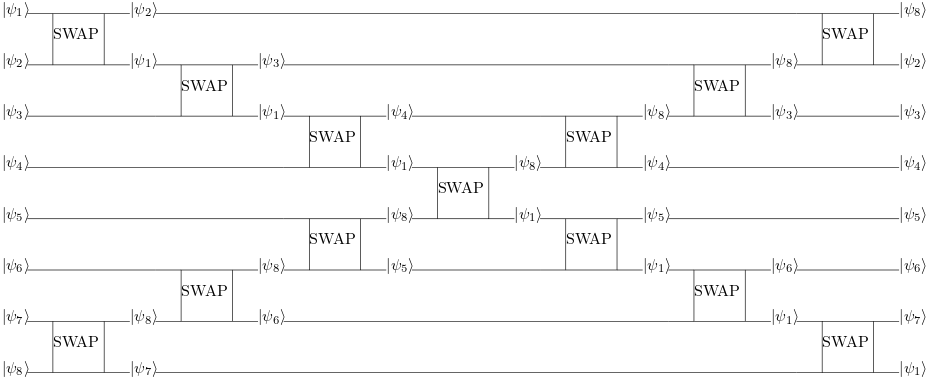
\includegraphics[width=6in]{modules/figs/m06/e12firstEighthSwap.png}
        \caption{Swapping the first and eighth qubits}
        \label{fig:first eighth swap}
    \end{figure}
    \item [3.] \textbf{Q.} With $n=2^{m}$ qubits, how many SWAP gates are needed to swap the first and last qubits? \textbf{A.}
    \begin{align*}
        2n-3
    \end{align*}
\end{enumerate}
 
\item[] \textbf{In-Class Exercise 13:} \textbf{Q.} Complete the remaining two steps in showing $\left(I \otimes \bar{C}_{\text {NOT }}\right) C C_{\text {NOT }}\left(I \otimes \bar{C}_{\text {NOT }}\right)$. \textbf{A.}
    \begin{align*}
        I \otimes \bar{C}_{N O T}=  & I \otimes(I \otimes|0\rangle\langle 0|+X \otimes| 1\rangle\langle 1|) \\
                                 =  & I \otimes I \otimes|0\rangle\langle 0|+I \otimes X \otimes| 1\rangle\langle 1| \\
                                 =  & (|00\rangle\langle 00|+| 01\rangle\langle 01|+| 10\rangle\langle 10|+| 11\rangle\langle 11|)
                                    \otimes|0\rangle\langle 0|\\
                                    & + (|00\rangle\langle 01|+| 01\rangle\langle 00|+| 10\rangle\langle 11|+| 11\rangle\langle 10|) \otimes|1\rangle\langle 1| \\
                                =   & |000\rangle\langle 000|+| 010\rangle\langle 010|+| 100\rangle\langle 100|+| 110\rangle\langle 110|\\
                                    & + |001\rangle\langle 011|+| 011\rangle\langle 001|+| 101\rangle\langle 111|+| 111\rangle\langle 101|\\
        C C_{\text{NOT}}        =   & |000\rangle\langle000|+|001\rangle\langle001|+|010\rangle\langle010|+|011\rangle\langle011|\\
                                    & + |100\rangle\langle100|+| 101\rangle\langle101|+|110\rangle\langle111|+|111\rangle\langle110|\\
        \left(I\otimes
        \bar{C}_{\text{NOT}}\right)
        C C_{\text{NOT}}
        \left(I\otimes
        \bar{C}_{\text{NOT}}\right) =   & (|000\rangle\langle000|+|010\rangle\langle010|+|100\rangle\langle100|+|110\rangle\langle110|\\
                                        & +|001\rangle\langle011|+|011\rangle\langle001|+|101\rangle\langle111|+|111\rangle\langle101|)\\
                                        & (|000\rangle\langle000|+|001\rangle\langle001|+|010\rangle\langle010|+|011\rangle\langle011|\\
                                        & +|100\rangle\langle100|+|101\rangle\langle101|+|110\rangle\langle111|+|111\rangle\langle110|)\\
                                        & (|000\rangle\langle000|+|010\rangle\langle010|+|100\rangle\langle100|+|110\rangle\langle110|\\
                                        & +|001\rangle\langle011|+|011\rangle\langle001|+|101\rangle\langle111|+|111\rangle\langle101|)\\
                                    =   & (|000\rangle\langle000|+|010\rangle\langle010|+|100\rangle\langle100|+|110\rangle\langle111|\\
                                        & +|001\rangle\langle011|+|011\rangle\langle001|+|101\rangle\langle110|+|111\rangle\langle101|)\\
                                        & (|000\rangle\langle000|+|010\rangle\langle010|+|100\rangle\langle100|+|110\rangle\langle110|\\
                                        & +|001\rangle\langle011|+|011\rangle\langle001|+|101\rangle\langle111|+|111\rangle\langle101|)\\
                                    =   & |000\rangle\langle000|+|010\rangle\langle010|+|100\rangle\langle100|+|110\rangle\langle101|\\
                                        & +|001\rangle\langle001|+|011\rangle\langle011|+|101\rangle\langle110|+|111\rangle\langle111|\\
    \end{align*}

\item[] \textbf{In-Class Exercise 14:} \textbf{Q.} Use the above idea to draw the circuit that converts $|110\rangle$ to $|001\rangle$. \textbf{A.} Figure \ref{fig:conversion}

    \begin{figure}
        \centering
        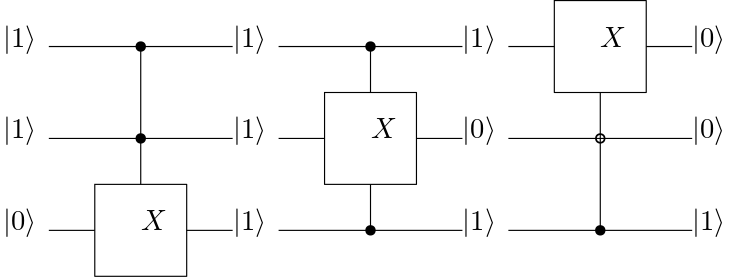
\includegraphics[width=5in]{modules/figs/m06/e14conversion.png}
        \caption{Circuit that converts $|110\rangle$ to $|001\rangle$}
        \label{fig:conversion}
    \end{figure}
    

\end{enumerate}
\end{document}